\chapter{Memetic Algorithm Configuration} % (fold)
\label{cha:evolutionary_algorithm_configuration}

The first thing to consider after having implemented the MA is figuring out what parameters should be used for it to perform well. Depending on the configuration, the MAs performance can be changed dramatically, and the quality of the results may vary. This chapter will look into the background for doing the configuration, outline the experimental plan for doing the tuning, show the results, and present a brief discussion on the outcome.

\section{Parameter Tuning} % (fold)
\label{sec:background_and_motivation}
Here the outline of how the parameters that should be used when running the MA will be discussed. There are several features that could be tweaked or enabled and disabled to alter how the MA works. For instance the population size and number of parents that get to reproduce each generation are values that can be adjusted. However, whether to use random mutation or memetic optimization is a choice of whether to use one of two implementations.

Some combinations of the parameters yield higher quality results faster (both in terms of actual time spent and number of generations passed before the output stabilizes, i.e., the program settles at a local optimum). Therefore, it is interesting to determine the best combination of parameters.

Initially these were the parameters for MA that the user could set:
\begin{itemize}
    \item How the genomes that would get to produce children were selected.
    \item How the nex generation would be generated from the current set of adults and children.
    \item Whether the fitness should evaluate one grand tour for one vehicle or consider a case where the given area should be divided among a set of vehicles.
    \item The maximal number of generations the algorithm should run for before terminating.
    \item If the algorithm gets stuck in a local optimum, for how many generations should it continue trying to get out of there before acknowledging that it is stuck and just returning the best answer it has.
    \item The number of individuals to have in the population at the beginning of a generation.
    \item How many individuals to select from the population that gets to mate each generation.
    \item How many pairs to make from the selected parents.
    \item If parents are selected tournament-style, what size (in terms of number of individuals) should each tournament group be.
    \item If parents are selected tournament-style, what should be the probability of selecting the best individual from each tournament group each iteration of the tournament.

\end{itemize}
% section background_and_motivation (end)

\section{Experimental Plan} % (fold)
\label{sec:experimental_plan}
% This should be the section about what we want to do, and why we want to do it
For the results to be as describing as possible, these tests should be run with the same input that one wishes to apply the MA to. That has the advantage of the results giving clear indications as to the computational time required, and one could come across a very good solution in the process. Also, if the structure of the search space influences the choice of parameters, it would become clear at this point. In this case, the search space would be the mapping of fitnesses to different permutations of visiting required elements in the underlying graph.

In the light of the research questions (specially RQ3) that would mean running the tests on a subsection of Trondheim with data from the NRDB. In practice, this posed several challenges. First of all, at the point in time where these tests could be done, the module structuring data from the NRDB was not complete. Second, if the assumption of that the structure of the search space might influence the outcome, it could be argued that different parts of Trondheim can be significantly different from each other. Which implies that for each section of the map that one wants to process, the parameters should be individually optimized. This choice would in turn lead to the dilemma of selecting the most representative part of the map, if such a thing is even possible. Third, if using real world data, there would be no way of knowing whether an optimal solution has been found, and evaluating the output beyond whether it is completely outlandish or somewhat reasonable. Fourth, it should be easy for a human to verify the output, both for correctness and whether the calculated fitness values make any sense.

Hence, to tackle the challenge of configuring the MA, a new data set was produced for the tuning. It can be found as a file named circle\_test.dat in the supplementary materials. The structure of the created graph is that of a directed cycle (as seen in Figure \ref{fig:ctgnaloc}). All of the arcs are required elements, which has several good qualities given the criteria above. First of all it is easy for a human to verify the output. There is only one global optimum, which is readily identifiable, visiting each node and arc in order exactly once. Furthermore, its fitness is trivial to calculate, as it is the sum of the traversal and servicing costs of all the elements exactly once. Any other ordering of the elements would lead to the circle being traversed more than once. Moreover, all the possible ways to order the required elements the MA could make would have a distinct fitness.

An example of an ideal solution to the circle test shown in Figure \ref{fig:ctgnaloc} would be the genome which is illustrated in Figure \ref{fig:bpgftscte}, which has a fitness value of 60.

\begin{figure}[H]
    \centerline{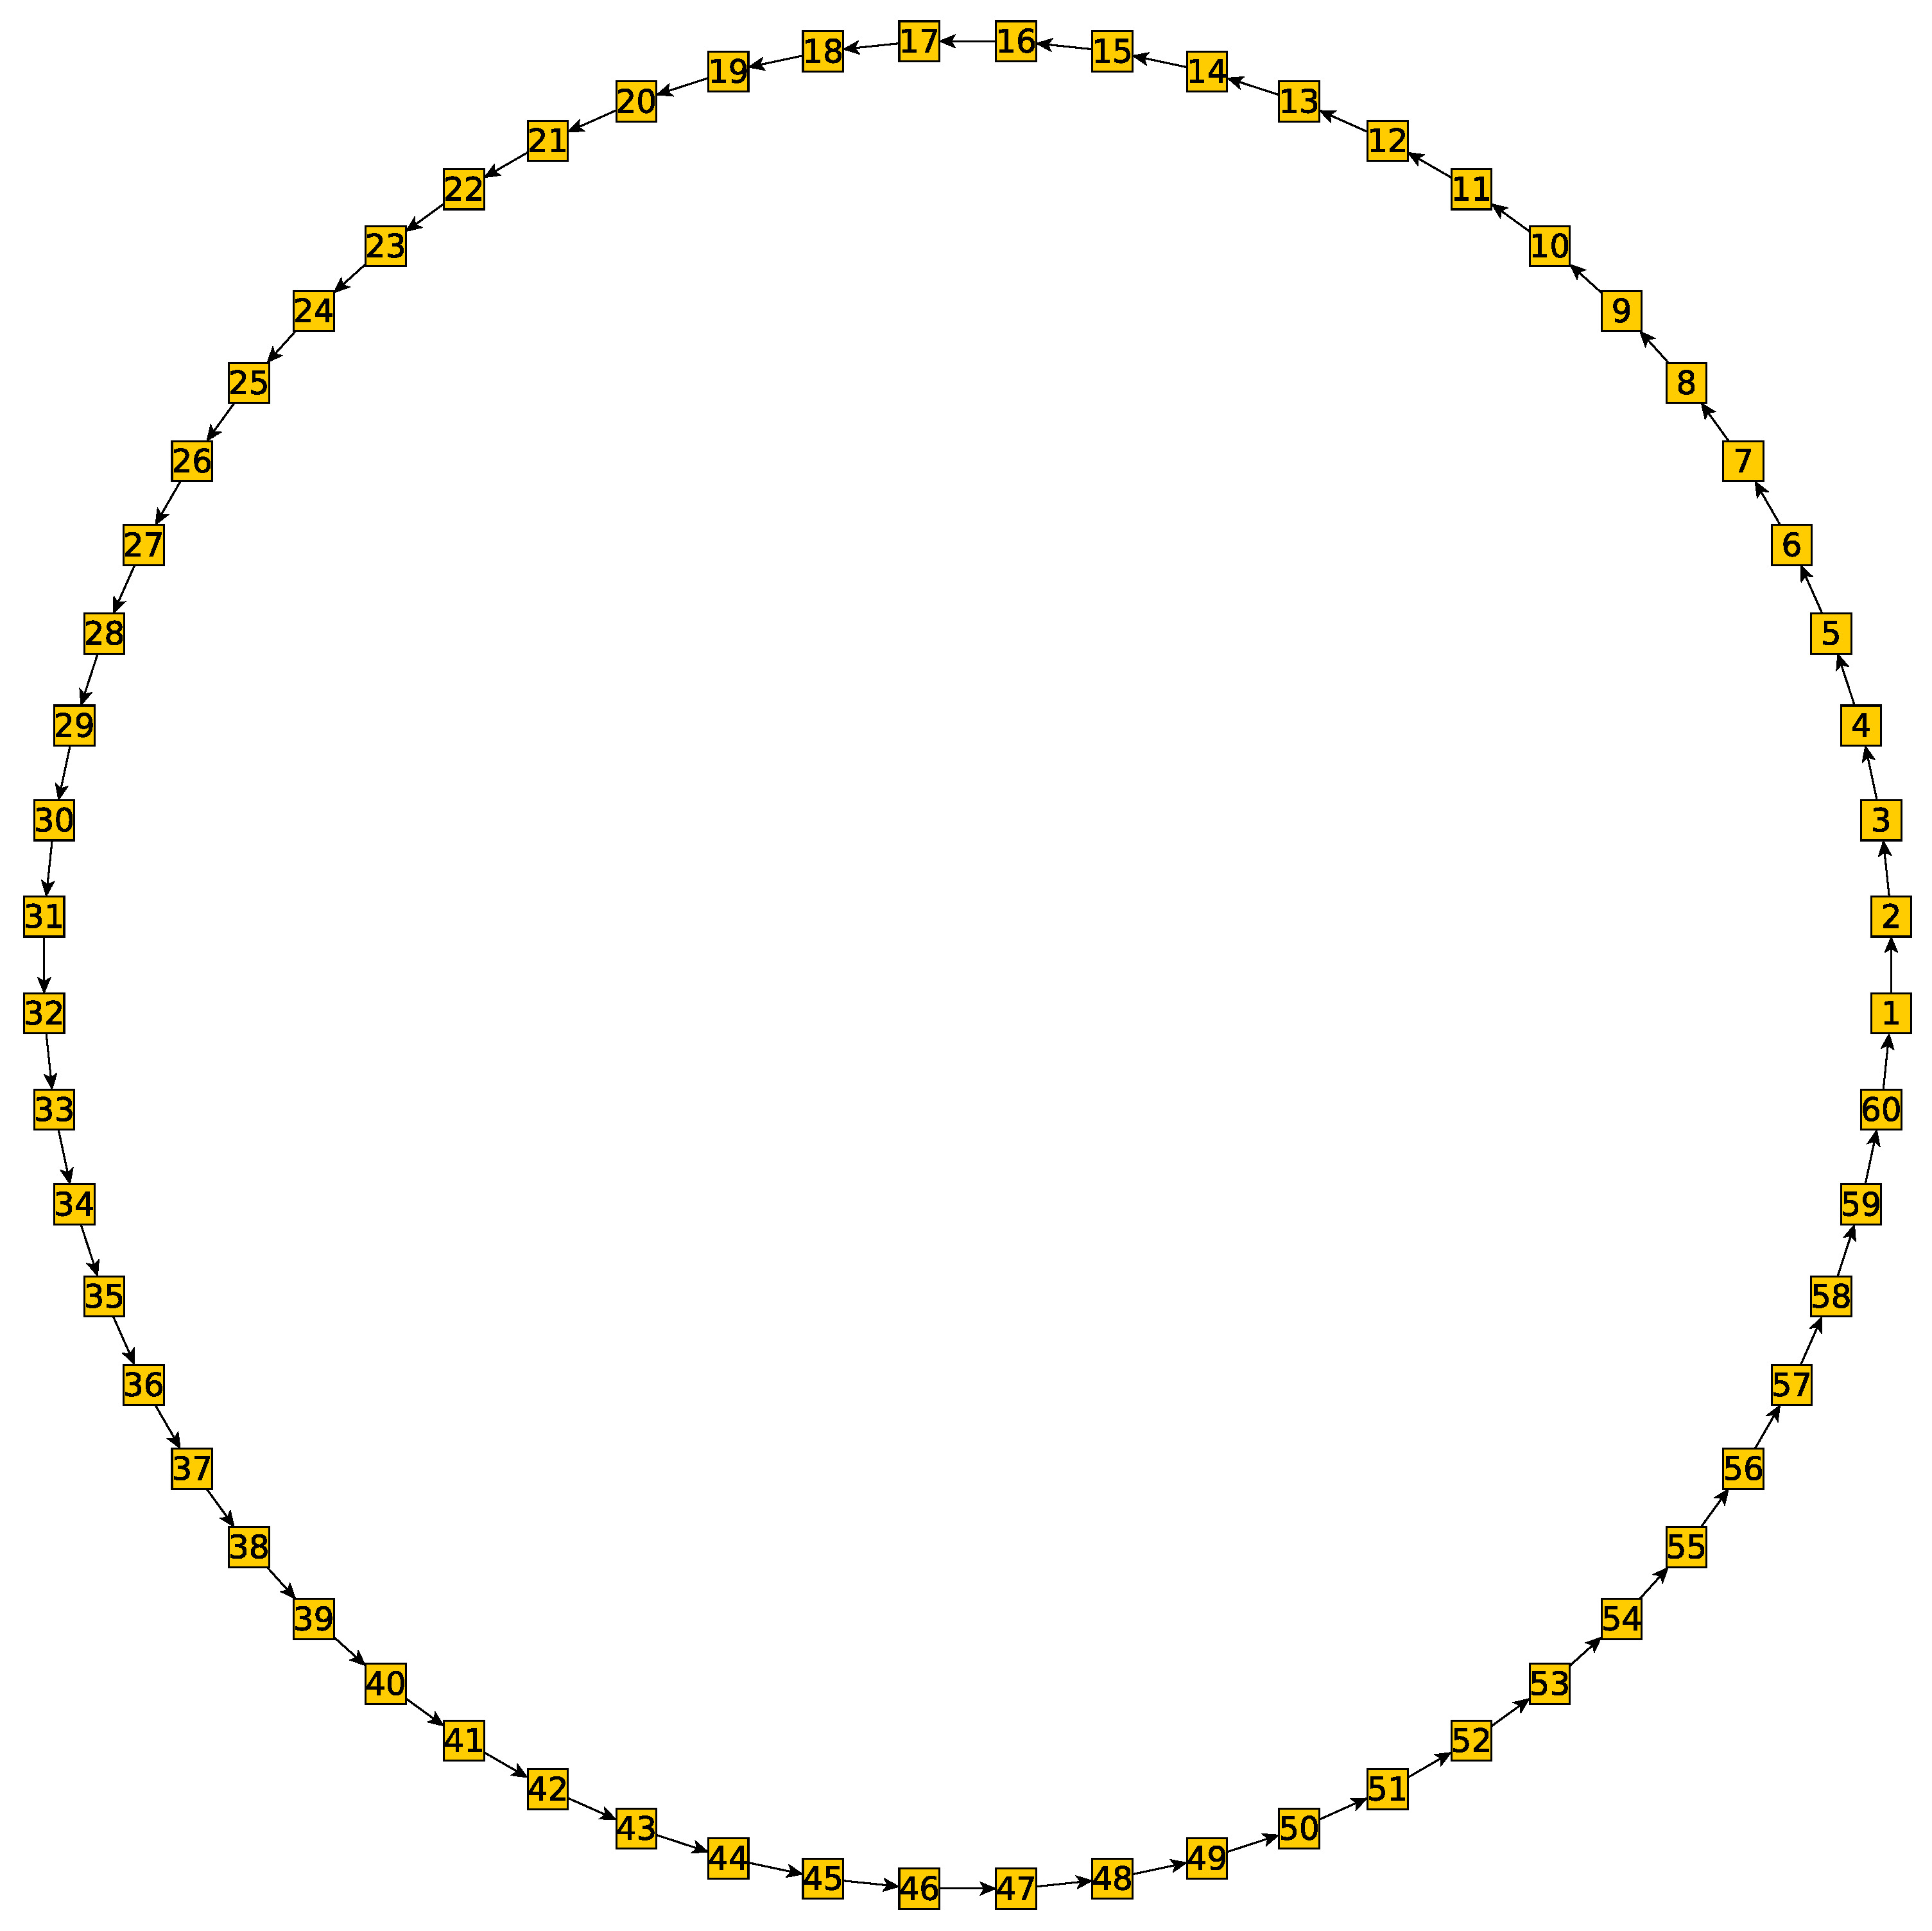
\includegraphics[width=\textwidth]{figures/CircleTests/CircleTestIllustrations/Circle_Test_Graph-No_arc_labels_or_costs.pdf}}
    \caption{Circle Test Graph example with no arc labels or costs drawn in}
    \label{fig:ctgnaloc}
\end{figure}

\begin{figure}[H]
    \noindent
    \fbox{
        \parbox{\textwidth}{
            A1, A2, A3, A4, A5, A6, A7, A8, A9, A10, A11, A12, A13, A14, A15, A16, A17, A18, A19, A20, A21, A22, A23, A24, A25, A26, A27, A28, A29, A30, A31, A32, A33, A34, A35, A36, A37, A38, A39, A40, A41, A42, A43, A44, A45, A46, A47, A48, A49, A50, A51, A52, A53, A54, A55, A56, A57, A58, A59, A60
        }
    }
    \caption{Best possible genome for the supplied Circle Test example}
    \label{fig:bpgftscte}
\end{figure}

While using the circle test data set might not give an exact answer to what configuration of the parameters is optimal, it still gives a usable prediction of what settings work in a general case with our implementation. Another limitation that is not addressed at this point is that it only makes sense to evaluate the test case as giant round trip completed by one vehicle. It could be adopted to facilitate testing splitting the graph between several vehicles by adding a depot node. It would have to be in the center, and edges that are not required to service would have to be made from it to all the nodes (as illustrated in Figure \ref{fig:ctgcdnaoeloc}). However that would add much complexity, and it would not be feasible to investigate it further at this point.

\begin{figure}[thbp]
    \centerline{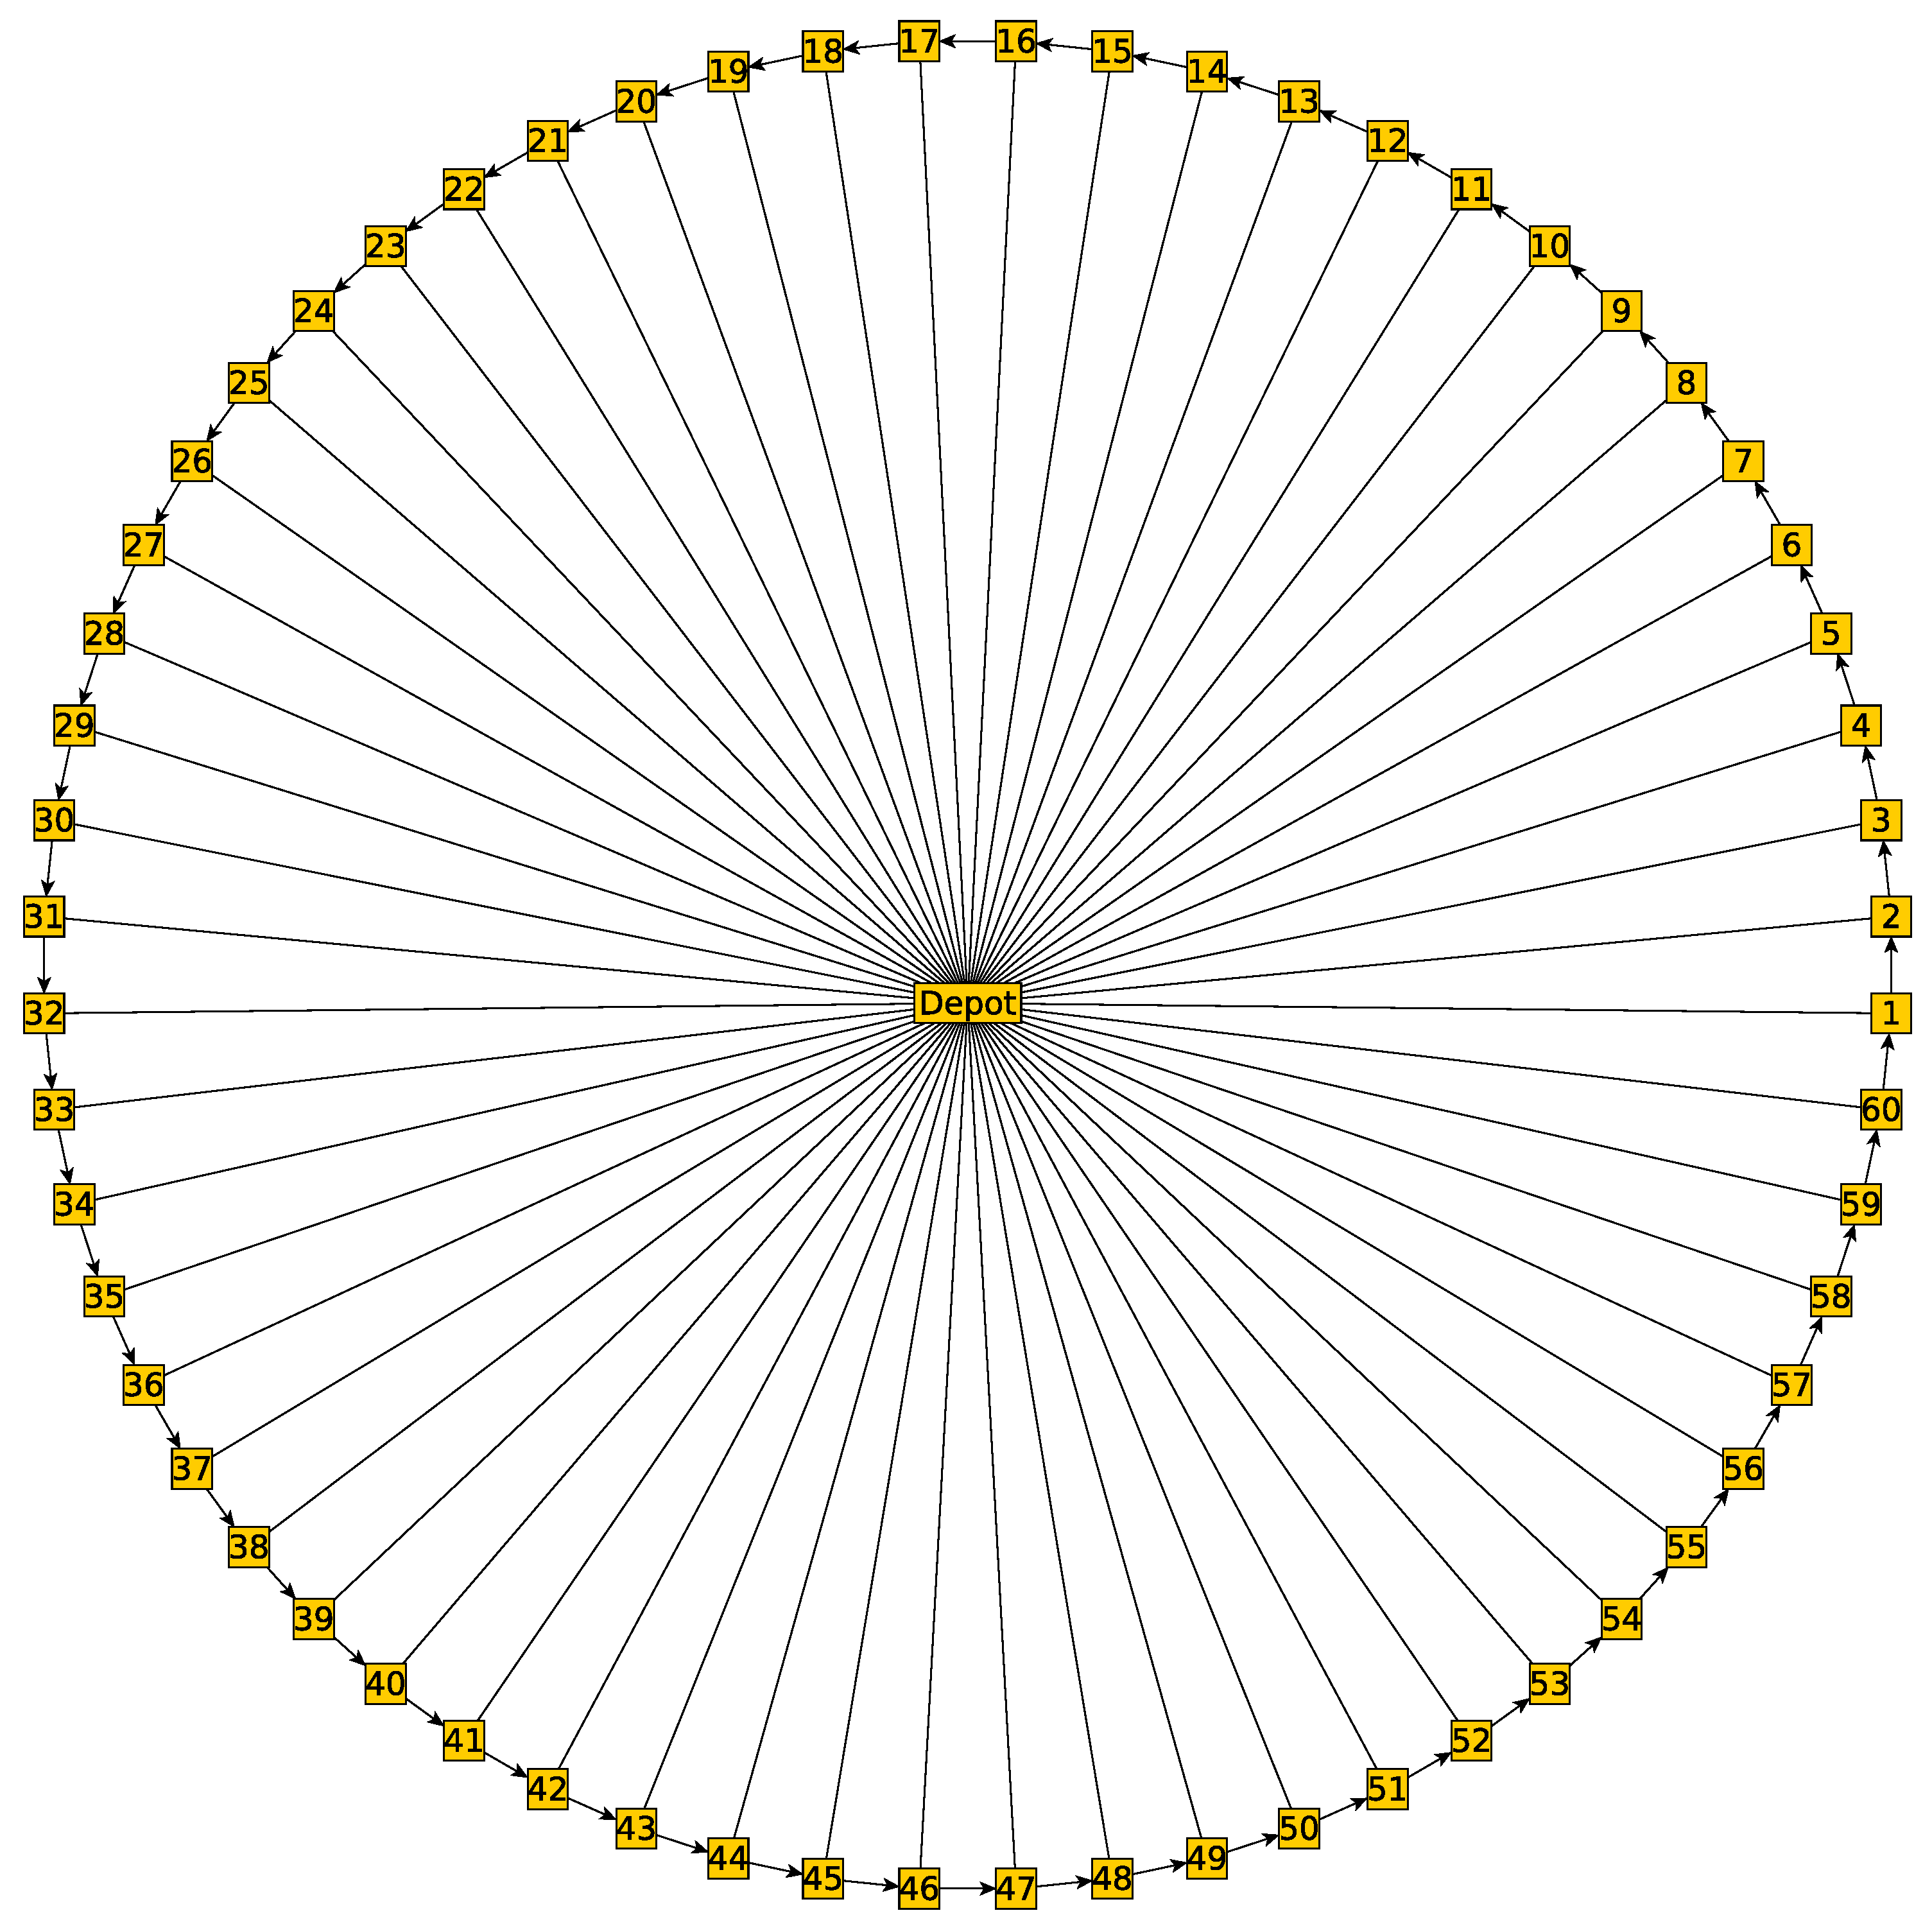
\includegraphics[width=\textwidth]{figures/CircleTests/CircleTestIllustrations/Circle_Test_Graph_Central_Depot-No_arc_or_edge_labels_or_costs.pdf}}
    \caption{Alternative Circle Test Graph example with depot node and no arc labels or costs drawn in}
    \label{fig:ctgcdnaoeloc}
\end{figure}

%Comment on memetics here?

% section experimental_plan (end)

\clearpage

\section{Experimental Setup} % (fold)
\label{sec:experimental_setup}
% This section should be about how we did the experiments, i.e., what parameters we used and so forth
The tuning of the MA was split into three parts; determining the population size, parent selection, and adult selection. 
For each part, a set of parameters to be tested were selected based on the author's previous experience with tuning EA's and the size of the problem at hand. Then each configuration was to be ran 30 times to gather data about the best results found with the configuration and the population averages. It was decided to let each configuration run for exactly 100000 generations, to make the results as comparable as possible. For each run, all the genotypes were initialized randomly.  Each 16th generation the best fitness of the population, the average fitness of the population, and the standard deviation of the fitness of the population at that point was recorded.

For determining the population size, it was decided to try population sizes corresponding to 10\%, 50\%, 100\%, and 200\% of the genome length. When testing it, uniform selection was used for parent selection and full generational replacement for the adult selection.

When trying different settings for the parent selection the size of the population is set at 200\% of the genome length. For the adult selection full generational replacement is used, as that allows for reuse of the results from the population size run for uniform selection.

When trying to find the best way to do the adult selection a population size of 200\% of the genome length, and fitness proportionate selection as the parent selection are used. When testing overproduction it was decided to make as many pairs as there are individuals in the population, i.e., it is produced twice as many children as there can be individuals surviving to next generation.

During the determination of whether random mutation or using hill climbing for mutation, a population size of 200\% of the genome length is used. The parent selection used is fitness proportionate selection, and the adult selection method is overproduction.

% section experimental_setup (end)

% \clearpage

\section{Results} % (fold)
\label{sec:results}

Now that the experimental plan has been outlined, in this section the results will be presented. First the initial results for the population size experiment will be shown. Then the outcome of using different parameters for the parent selection is going to be laid out. After that, the experimental results when testing different configurations for mutation are going to be presented. Finally, the results from a follow-up experiment on the population size will be shown. All the relevant graphs can be found in Appendix \ref{cha:memetic_algorithm_tunin_results}.

\subsection{Population Size} % (fold)
\label{sub:population_size}

When observing the results from the population size test runs, it can be noticed that that a lower population size yields better results. Figure \ref{fig:ctpab} in Appendix \ref{sec:population_size_testing_results} shows that the larger populations perform noticeably worse. The largest population (120 individuals) gets a fitness value of around 700 by the end of the runs while the smallest population size (6 individuals) ends up with a fitness of about 600.

A possible reason for this is that uniform selection combined with full generational replacement is not biased in any way. The lack of steering makes it very random in terms of that the fitness of the individuals in the existing population will not affect future generations. The population will, however, be influenced by the previous generations in terms of that their genomes will be combinations of previous genomes with mutations.

A possible explanation then could be in that the best individual from each generation is kept and is injected in place of the worst one at the end of each generation. The insertion will have an enormous impact on a tiny population of only six individuals, effectively dragging the population towards the currently best. However, as population sizes increase the best individual, and its offspring have less impact on the average of the population.

This effect should be offset by introducing bias in the population towards that the individuals with better fitness have a better chance at impacting future generations. However, to be certain that this is a quirk of combining uniform selection, full generational mixing, and the constant reintroduction of the previous best single individual at the cost of the currently worst, more testing should be done. Therefore, a control experiment for parent size using another form of parent selection and generational replacement is set up.

\subsection{Parent Selection} % (fold)
\label{sub:parent_selection}

In Figure \ref{fig:ctpsab} in Appendix \ref{sec:parent_selection_results} it can be seen that fitness proportionate selection is clearly better than the tournament selection, which in turn finds better results on average than uniform selection. Their final fitnesses are just below 500, a bit above 500, and around 700 respectively. The averages fitness of each populations average seems to decrease quickly before beginning to decrease more slowly for tournament and fitness proportionate selection while the uniform selection shows only a very slow improvement over time.

\subsection{Adult Selection} % (fold)
\label{sub:adult_selection}

When looking at the results for the adult selection in Figure \ref{fig:ctasab} in Appendix \ref{sec:adult_selection_results}, the most striking thing is the completely flat curve for the elitist mixing average best. It indicates that there on average is no improvement at all in the best solutions found when using it as adult selection. This can be explained by observing that the average standard deviation in each population is 0 (Figure \ref{fig:ctasasd}, Appendix \ref{sec:adult_selection_results}). Coupled with that the average fitness of the population being stuck on a single value in Figure \ref{fig:ctasaa} from Appendix \ref{sec:adult_selection_results}, it indicates that all the individuals in the population have the same fitness. What seems to have happened is that the population has become stuck in a local optimum, and all the individuals it produces are exact copies of the currently best found solution.

When looking for what adult selection gives the best output according to these results both overproduction and random mixing give better results than elitist mixing and overproduction yields slightly better results than random mixing.

\subsection{Mutation Types} % (fold)
\label{sub:mutation_types}

As seen from figures \ref{fig:ctmab} and \ref{fig:ctmaa} in Appendix \ref{sec:mutation_types_results} the memetic improvement yields better results than when doing random mutation. Adding a memetically improved child to the children before the adult selection seems to make little difference though it reaches a somewhat better solutions a little bit earlier than when not adding it. For both memetic approaches the fitness value tends to get as good as just below 400 in the long run, as seen in Figure \ref{fig:ctmab} from Appendix \ref{sec:mutation_types_results}.

Figure \ref{fig:ctmasd} in Appendix \ref{sec:mutation_types_results} shows that the diversity of the population is somewhat lower when doing memetic improvement instead of random mutation.

\subsection{Population Size Control} % (fold)
\label{sub:population_size_control}

Due to the unexpected results in the population size tests (Chapter \ref{sub:population_size}), it was decided to look into whether the effects of the population size that appeared could be explained by the lack of elitism. Especially because the choice of using uniform parent selection and full generational replacement removes any form of elitism that normally arises in the GA/MA process. A control test was set up, where again 30 populations were run, but this time with fitness scaling selection and overproduction with twice as many children as the population size.

The results that were obtained are according to the predictions about a population yielding better output as its size increases. Also, the results indicate that the behavior when not guiding the development of the population in any direction actively is heavily influenced by the reuse of the best individual. 

A larger population gives better results, but as the populations grow very large, there are diminishing returns on expanding it further. As seen in Figure \ref{fig:cpscab} in Appendix \ref{sec:population_size_control_results} the largest population gives only marginally better results than the second largest population. Which in turn gives somewhat better results than the third largest population, which gives a lot better results than the smallest population.

\section{Summary of Parameter Tuning Results} % (fold)
\label{sec:evaluation_and_conclusion}

The above experiments lead us to the following conclusions about the parameters for the MA. Chapter \ref{sub:parent_selection} indicated that the best parent selection method for the algorithm is fitness proportionate selection. As for the adult selection, Chapter \ref{sub:adult_selection} shows that overproduction is the adult selection type that gives the best fitnesses in our implementation. When it comes to the mutation tests in Chapter \ref{sub:mutation_types}, it can be seen that memetic improvement gives much better results than random mutation.

Chapter \ref{sub:population_size_control} shows that larger populations yield better results, but that increasing the size has diminishing returns. It also shows that a population size of 200\% the length of the genome is not much better than a population size equivalent to 100\% the length of the genome. The findings in the chapter contradict the findings from Chapter \ref{sub:population_size}, but they indicate that those findings are arising due to a specific combination of factors. A smaller population happens to be better in the following situation:

\begin{compactitem}
    \item The previous best individual is reintroduced each generation.
    \item The portion of the population the best individual constitutes grows larger as populations grow smaller.
    \item No other form of elitism or directing of the populations development is present.
\end{compactitem}

None of the configurations found an ideal solution with a fitness value of 60. The best fitness values the MA got were about 400 (found when doing the mutation configurations in Chapter \ref{sub:mutation_types}) which is not too bad. The found fitness value indicates that the MA gives a solution that goes $\frac{400}{60} = 6.\overline{66} \approx 7$ times more than it needs around the circle. Considering that this can be achieved by switching the order of 7 pairs in the circle the quality of the solutions while not optimal are still acceptable.

Overall the experiments ran smoothly, usable results were obtained, and more importantly all of the results above are 100\% reproducible because all the configurations and random-seeds of each run of each experiment were kept.

There are several things that could be improved. A test that also tests splitting would be better. Using real-world test data would give indications as to running time, which would make it better in itself. Furthermore, that could provide more parameters, which in turn could make the MA perform even better. Another significant limitation is that other configurations of the tournament selection were not looked into.

{
\rowcolors{2}{gray!15}{white}
\begin{table}[tbph]
\centering
\begin{tabular}{ll}
\toprule
\textbf{MA Parameter} & \textbf{Best found setting}     \\ \midrule
Parent selection      & Fitness proportionate selection \\
Adult selection       & Overproduction                  \\
Mutation type         & Memetic improvement             \\
Population size       & 200\%                           \\ \bottomrule
\end{tabular}
\caption{The tunable parameters in the MA and what settings were found to give the best results}
\label{tab:parameter_table}
\end{table}
}
% section evaluation_and_conclusion (end)
% chapter evolutionary_algorithm_configuration (end)

\cleardoublepage
